\documentclass[]{article}
\usepackage{xeCJK}
\usepackage[colorlinks,linkcolor=green, anchorcolor=green, citecolor=green]{hyperref}
\usepackage{graphicx}
\usepackage{subcaption}
\usepackage{amsmath}


%opening
\title{深度解读条件随机场\footnote{在自然语言处理领域,由于文本具有序列性,实际只讨论条件随机场(Conditional Random Field, CRF)的一个特例,即线性链条件随机场(Linear Chain CRF)。}}
\author{Yang Fu}

\begin{document}

\maketitle

\begin{abstract}
CRF是概率图模型中极具代表性的概率无向图模型,常用于命名实体识别等序列标注任务。
CRF模型的表达式是对数线性函数,参数包括特征函数及其权重。
训练时,基于前向-后向算法计算正则化后的概率值,然后基于极大似然估计训练模型参数;
推理时,基于维特比算法计算给定观测序列下条件概率最大的标签序列。
CRF的实现版本有两种,传统机器学习实现版本支持人工显式地定义特征模板,深度学习实现版本在所有位置上共享特征函数及其权重。
相比Softmax,CRF接受标签转移约束,基于全局归一化预测,彻底解决了标签不一致的问题,缺点是归一化因子计算量较大,同时不能很好处理嵌套和不连续实体。
\end{abstract}

\section{理论部分}

\subsection{模型表达式}

给定序列$x$,CRF预测标签序列$y$的条件概率$P(y|x)$为:

\begin{equation}\label{key}
	P(y|x) = \frac{1}{Z(x)}exp \bigg(\sum_{i,k}\lambda_k t_k(y_{i-1}, y_i, x, i) + \sum_{i, l}\mu_l s_l(y_i, x, i)\bigg)
\end{equation}

\begin{equation}\label{key}
	Z(x) = \sum_{y} exp\bigg(\sum_{i,k} \lambda_k t_k(y_{i-1}, y_i, x, i) + \sum_{i,l} \mu_l s_l(y_i, x, i)\bigg)
\end{equation}

\begin{itemize}
	\item $Z(x)$是归一化因子,使得$\sum_y p(y|x) = 1$,实现了全局归一化;
	\item exp()的角色是势函数;
	\item $t_k$和$s_l$分别是状态转移特征函数和状态特征函数,取值为0或1,$\lambda_k$和$\mu_l$是对应特征函数的权重;
\end{itemize}

接下来从概率无向图模型开始,逐步推导CRF模型表达式。

\subsection{推导过程}

概率无向图模型又称马尔可夫随机场,它要求$P(Y)$必须满足成对、局部、全局马尔可夫性,然后根据Hammersley-Clifford定理,概率无向图模型的联合概率分布$P(Y)$可以分解成规范化的最大团的势函数乘积\footnote{这里暂不深究Hammersley-Clifford定理,只需明确概率无向图模型的联合概率是由图中最大团的势函数相乘得到的。关于最大团的定义可以查阅图论。}。

在马尔可夫随机场的基础上引入随机变量X,Y保持为马尔可夫随机场,则给定X条件下Y的条件概率$P(Y|X)$即表示条件随机场。特殊地,如果Y具有链式结构,便得到线性链条件随机场。由于Y仍旧满足马尔可夫性,有$P(Y_v|X, Y_w, w \neq v) = P(Y_v|X, Y_v, w \sim v)$,其中$\sim$表示相邻。则线性链条件随机场的条件概率可表示为:

\begin{equation}\label{key}
	P(Y_i|X, Y_1, ..., Y_{i-1}, Y_{i+1}, ..., Y_n) = P(Y_i|X, Y_{i-1}, Y_{i+1})
\end{equation}

Fig 1展示了两种形式的线性链条件随机场。由于线性链条件随机场的最大团就是相邻两个结点的集合。而通过对这两张图进行内部比较,可以发现左边的图更为特殊,因为X和Y具有相同的结构。现实中,比如对于NER问题,对一个文本序列进行序列标注,都一般假设X和Y具有相同结构,满足左边的那张图。

\begin{figure}[h]
	\begin{subfigure}{0.5\textwidth}
		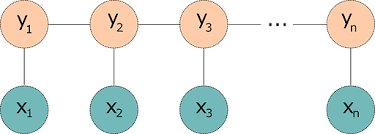
\includegraphics[width=0.9\linewidth]{../images/crf_2}
		\caption{X和Y都具有链式结构}
		\label{fig:subim2}
	\end{subfigure}
	\begin{subfigure}{0.5\textwidth}
		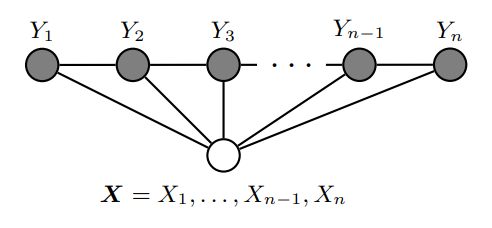
\includegraphics[width=0.9\linewidth]{../images/crf} 
		\caption{仅Y具有链式结构}
		\label{fig:subim1}
	\end{subfigure}
\caption{CRF架构图}
\label{fig:image2}
\end{figure}

基于两种形式的最大团,CRF分别定义状态转移特征函数$t_k(y_{i-1}, y_i, x, i)$和状态特征函数$s_l(y_i, x, i)$,并给它们分配了权重。这两种特征函数分别描述了状态转移概率和发射概率。以特征函数$t_1$为例:

\begin{equation}\label{key}
	t1(y_{i-1}=1, y_i=2, x, i) = 1, \quad i=2, 3
\end{equation}

特征函数$t_1$的含义是当$i=2$或$3$时,如果$y_{i-1}=1, y_{i}=2$成立,特征函数$t_1$取1,否则$t_1$取0.

在Hammersley-Clifford定理中,势函数必须是非负函数,CRF采用exp作为势函数,最大团的势函数的乘积就变成指数上的累加。

于是,便可得到线性链条件随机场的模型表达式:

\begin{equation}\label{key}
	P(y|x) = \frac{1}{Z(x)}exp(\sum_{i,k}\lambda_k t_k(y_{i-1}, y_i, x, i) + \sum_{i, l}\mu_l s_l(y_i, x, i))
\end{equation}

这里有一个细节值得注意:$i$和$k/l$分别是位置编号和特征函数编号,它们是分开的!换句话说,每个位置上都存在多种特征函数,而一个特征函数又作用在整个序列$y$上。

\subsection{CRF的矩阵表达形式}

将两种特征函数统一为$f_k(y, x)$,得到上一节模型表达式的简化表达:

\begin{equation}\label{key}
	P(y|x) = \frac{1}{Z(x)}exp(\sum_{k=1}^K w_kf_k(y, x))
\end{equation}

\begin{equation}\label{key}
	f_k(y, x) = \sum_{i=1}^L f_k(y_{i-1}, y_i, x, i)
\end{equation}

可以看到,$f_k(y, x)$是单个特征函数在整个序列上的取值,$P(y|x)$是所有特征函数与权重的加权和。这里的特征函数有$K$个,是两种特征函数的数量和,位置则是从$1$到$L$。

接下来,尝试将其转化成向量形式\footnote{这里的$\cdot$表示内积。}:

\begin{equation}\label{key}
	P_w(y|x) = \frac{exp(w \cdot F(y, x))}{Z_w(x)}
\end{equation}

\begin{equation}\label{key}
	w = (w_1, w_2, ..., w_K)^T
\end{equation}

\begin{equation}\label{key}
	F(y, x) = (f_1(y, x), f_2(y, x), ..., f_K(y, x))^T
\end{equation}

将表达式继续简化为矩阵表示形式。假设标签集合为$\{v_1, v_2, ..., v_c\}$,在位置$i$处定义一个$c$阶矩阵随机变量:

\begin{align*}		
	M_i(x) &= [M_i(y_{i-1}, y_i, x)] \\
		&= \begin{bmatrix}
		M_i(y_{i-1}=v_1, y_i=v_1|x) & M_i(y_{i-1}=v_1, y_i=v_2|x) & \cdots & M_i(y_{i-1}=v_1, y_i=v_c|x)\\
		M_i(y_{i-1}=v_2, y_i=v_1|x) & M_i(y_{i-1}=v_2, y_i=v_2|x) & \cdots & M_i(y_{i-1}=v_2, y_i=v_c|x)\\
		\vdots & \vdots & \ddots & \vdots\\
		M_i(y_{i-1}=v_m, y_i=v_1|x) & M_i(y_{i-1}=v_c, y_i=v_2|x) & \cdots & M_i(y_{i-1}=v_m, y_i=v_c|x)
	\end{bmatrix}
\end{align*}

其中

\begin{equation}\label{key}
	M_i(y_{i-1}, y_i, x) = exp(W_i(y_{i-1}, y_i|x))
\end{equation}

\begin{equation}\label{key}
	W_i(y_{i-1}, y_i|x) = \sum_{k=1}^K w_kf_k(y_{i-1}, y_i, x, i)
\end{equation}

如果考虑起始和终止标签,标签序列$y=\{y_0, y_1, ..., y_{L+1}\} = \{start, y_1, y_2, ..., y_L, stop\}$的条件概率为:

\begin{equation}\label{key}
	P_w(y|x) = \frac{1}{Z_w(x)}\prod_{i=1}^{L+1} M_i(y_{i-1}, y_i|x)
\end{equation}

这里的分子就是当前标签序列$y$的预测分数。所有可能的标签序列共有$L^C$种,归一化因子$Z_w(x)$是以start为起点,以stop为终点通过状态的所有路径的非规范化概率$\prod_{i=1}^{n+1} M_i(y_{i-1}, y_i|x)$之和。

综上,考虑start和stop的CRF模型的参数量是$(L+1)*C*C$,但是实际上,tensorflow和pytorch实现代码中,$M_i(x)$在所有位置上共享,因而参数量为$C*C$.

\section{训练}

\section{推导}

\section{实现}

\bibliographystyle{unsrt}
\bibliography{crf}
\end{document}
